\documentclass[a4paper,14pt]{report}
\usepackage{graphicx}
\usepackage{hyperref}
\usepackage{amsmath}
\usepackage{caption}
\usepackage{listings}
\usepackage{float}
\usepackage{cite}

\begin{document}
% Cover Page
\begin{titlepage}
    \begin{center}
        
\includegraphics[width=0.2\textwidth]{Images/logo.png}\\[1cm]
        \Large
        \textbf{Khulna University of Engineering \& Technology}\\
        Department of Computer Science and Engineering\\
        \vspace{1cm}
        \textbf{Topic: Fake Image Detection} \\           
        CSE 4120: Technical Writing \& Seminar\\
        \vspace{1cm}    
        \textbf{Instructed by:}\\
        Dr. K. M. Azharul Hasan\\
        Professor,\\ Department of CSE, KUET\\
        Sunanda Das\\
        Assistant Professor,\\ Department of CSE, KUET\\
        \vspace{1cm}
        \textbf{Submitted by:}\\
        Nushrat Tarmin Meem\\
        Roll: \textbf{1907083}\\
        Date of Submission: 03.06.2024 
    \end{center}
\end{titlepage}

% Table of Contents
\tableofcontents
\newpage
% List of Tables
\listoftables
\newpage
% List of Figures
\listoffigures
\newpage

% Main Content
\chapter*{Abstract}
%\addcontentsline{toc}{chapter}{Abstract}
Now a days, due to excessive use of internet, a major concern has been detected in case of social media along with security issues for proper identification. Besides this, fake images or AI generated images have already taken a large portion on the internet for which it's a very difficult problem in fields like journalism, forensics, and social media. To solve this issue, in total three papers from different sources have been studied regarding this and compared with each other for driving a conclusion to find out which one is the optimal solution for detecting fake images according to accuracy and also some parameter comparison of image processing and computer vision techniques. Different networks including NAFID \cite{1} , CLIP:ViT \cite{2} , Robust Hashing \cite{3}  methods have been compared to each other. Above all, future research directions have been discussed focusing on the need for larger and more diverse datasets, real-time detection capabilities and the development of methods that can adapt to the evolving techniques of image manipulation and most importantly can detect AI or GAN generated images.

\chapter{Introduction}
The production and manipulation of phony photographs has grown in sophistication in recent years, creating serious problems for forensics, social media, and journalism, among other fields. The demand for efficient detection systems grows as realistic false picture creation capabilities advance. For journalism to deliver accurate news reporting, picture authenticity is crucial. Fake photos have the potential to mislead people and erode public confidence in media outlets. In forensics, the capacity to discriminate between authentic and altered photographs is essential to maintaining the integrity of investigations and the administration of justice. Fake photos can spread quickly and extensively on social media platforms, affecting public opinion and disseminating false information. This can be quite harmful.\\
Multiple sophisticated techniques for detecting phony images have been developed in order to overcome these problems. Neural Architecture for Fake picture Detection (NAFID) \cite{1} is one such technique that uses deep learning to automatically detect anomalies in picture data. Through the examination of an image's underlying features, NAFID \cite{1} is able to identify forgeries that the human eye could miss. On the otherhand, CLIP-ViT \cite{2} , or Contrastive Language-Image Pre-training mixed with Vision Transformers, is another innovative technique. This method offers an effective framework for deciphering and examining the connection between visuals and their written explanations. Through the integration of both textual and visual data, CLIP-ViT \cite{2} improves and broadens the detection process. It can detect differences between the text that goes with an image and the content of the image itself, which is especially helpful for identifying deepfakes and other complex image manipulations. Lastly robust hashing \cite{3} methods provide an alternative by producing distinct hashes, or digital fingerprints, for each image. By comparing photos, these hashes make it possible to find any changes or duplication. This technique works very well for confirming the legitimacy of photos and making sure they haven't been altered since they were taken.\\
By integrating these advanced techniques—NAFID \cite{1}, CLIP-ViT \cite{2}, and robust hashing \cite{3} —the accuracy and reliability of fake image detection can be significantly improved. These methods complement each other, providing a multi-faceted approach to detecting fake images.

\chapter{Background/Problem Statement}
\section{Background}
The development of advanced digital technology has completely changed how we produce, edit, and distribute photos. Digital image manipulation is a serious danger to a number of industries, including social networking, forensics, and journalism. In the field of journalism, the veracity of visual content is crucial to the trustworthiness of news stories. Forensics relies heavily on picture evidence integrity to ensure that investigations are accurate and that justice is served. The quick sharing and consumption of photos on social media platforms makes them especially susceptible to the propagation of false information via phony photographs.
\section{Problem Statement}
Fake image identification is a complicated and serious topic. The volume of photos created and exchanged every day, along with the growing sophistication of image alteration techniques, make traditional methods of image verification, including expert manual examination, insufficient. Deepfakes and other contemporary fake images are produced with sophisticated machine learning algorithms that yield remarkably lifelike results, rendering them undetectable to the unaided eye.\\
Finding minute irregularities in the image data that point to tampering is one of the main problems in false image detection. Furthermore, reliable techniques are required to continuously confirm the legitimacy of photos, guaranteeing that any modifications are precisely detected. In order to tackle these issues, scientists have created a number of sophisticated techniques for identifying phony images. To sum up, the identification of counterfeit photographs is a serious problem that necessitates sophisticated, automated solutions in order to guarantee the legitimacy of visual material in a variety of contexts. In this continuous fight against image manipulation, the creation and application of methods like NAFID, CLIP-ViT, and strong hashing represent important advancements.

\chapter{Review of Literature}
Numerous studies have been conducted in the realm of fake image detection, each focusing on different aspects and techniques to identify forgeries. Some works have concentrated on detecting forgery clues in facial features, head poses, blinking patterns, or skin colors. For instance, studies in this field have demonstrated that irregularities in these components may serve as a red flag for photos that have been altered \cite{4} \cite{5} \cite{6}. These investigations use small, sometimes undetectable differences in head movements, atypical skin tone distributions, odd blinking patterns, and facial expression variances \cite{7} \cite{8} to detect bogus photos.\\
Apart from these physical and facial clues, additional study endeavors have focused on identifying conspicuous alterations in photographs. Observable distortions or alterations that can be found using conventional image processing techniques may be among these changes \cite{6} \cite{9}. These techniques sometimes entail comparing an image to well-known benchmarks or identifying anomalies that may indicate modification by applying basic heuristics.\\
Still, detecting photographs with slight distortions is one of the major hurdles in bogus image detection. Subtle modifications require more advanced procedures to detect, whereas blatant changes can be relatively easier to discover. Studies have brought attention to the shortcomings of existing detection techniques in these kinds of situations, highlighting the necessity for more sophisticated and sensitive procedures \cite{10} \cite{11} \cite{15} \cite{16}.\\
Modification of texture information has been another important area of attention. Researchers have created techniques to identify texture changes in photos, which can be a clear indicator of image manipulation. These methods seek to identify changes that might otherwise go undetected by examining the regularity and authenticity of texture patterns \cite{13} \cite{16}.\\
The detection of Generative Adversarial Network (GAN) or AI-generated fake images presents an even greater challenge. GANs can produce highly realistic images that are difficult to distinguish from genuine ones. Research in this domain has been dedicated to developing advanced algorithms and techniques specifically designed to detect GAN-generated fakes, recognizing the unique patterns and anomalies that these AI-generated images exhibit \cite{10} \cite{12} \cite{14} \cite{18}.\\
These various approaches collectively contribute to the advancement of fake image detection, addressing the complexities and evolving nature of image manipulation.

\chapter{Methodology}
\section{Paper 1: New Finding and Unified Framework for Fake Image Detection}
Detecting fake images requires a multifaceted approach, blending traditional image analysis methods with cutting-edge machine learning techniques. First, a heterogeneous dataset comprising real and artificial images is put together. The photos are standardized and any possible interference is eliminated through preprocessing. After that, features are extracted from the images in order to identify statistical, structural, and semantic properties. Based on these features, machine learning models—which include supervised and unsupervised algorithms—are then used to learn and distinguish between authentic and fraudulent images. 
\begin{figure}[H]
    \centering
    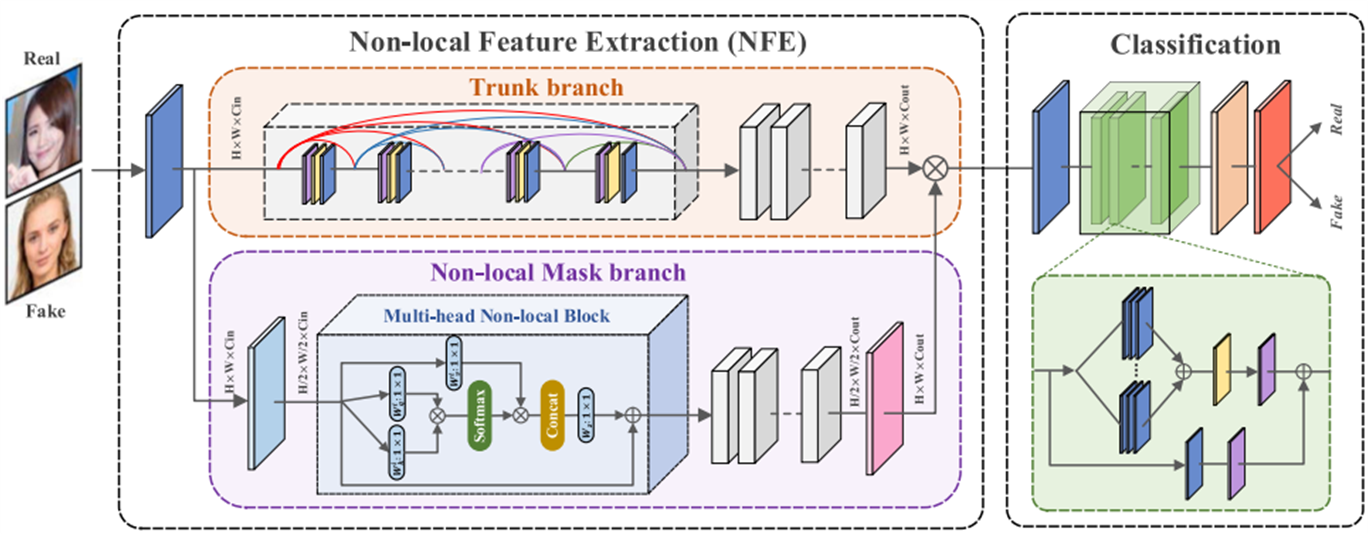
\includegraphics[width=0.8\textwidth]{Images/method_paper1.png}
    \caption{NAFID network for face forgery detection (Paper 1)}
    \label{fig:rainy_clean}
\end{figure}
The overall methodology of this paper has been shown within the diagrams of figure \ref{fig:methodology}.
It is basically understanding how fake images are created—specifically, through face generation and manipulation techniques using Generative Adversarial Networks (GANs) \cite{10} \cite{18} — motivates the suggested method for detecting fake images, known as NAFID. The approach takes advantage of the finding that, as a result of the generation process, GAN-generated fake faces frequently show stronger non-local self-similarity than real faces by examining their features. As a result of their stronger non-local self-similarity, fake faces typically have higher Peak Signal-to-Noise Ratio (PSNR) values after denoising. Additionally, the PSNR distribution of fake faces is more concentrated than that of actual faces, indicating less fluctuation. The NFE module is composed of a non-local mask branch that uses multi-head attention to capture various non-local information and a trunk branch for feature extraction. For the purpose of final detection, the collected non-local features are then input into a ResNeXt classification network. This method uses the unique features of GAN-generated \cite{10} \cite{18} fake faces in contrast to real ones to show how easy yet effective it can be to identify phony photos
\section{Paper 2: Towards Universal Fake Image Detectors that Generalize Across Generative Models}
In order to detect fake images, this paper has proposed a methodology that makes use of a feature space that has not been specifically trained for real or fake image classification. The approach does away with the need to train a neural network to discriminate between real and fake classes by utilizing a pre-trained CLIP visual encoder that has been exposed to a sizable dataset of image-text pairs. This encoder was chosen for its ability to capture low-level image details and its wide exposure to a variety of visual content. This paper makes use of the nearest neighbor and linear classification techniques.
\begin{figure}[H]
    \centering
    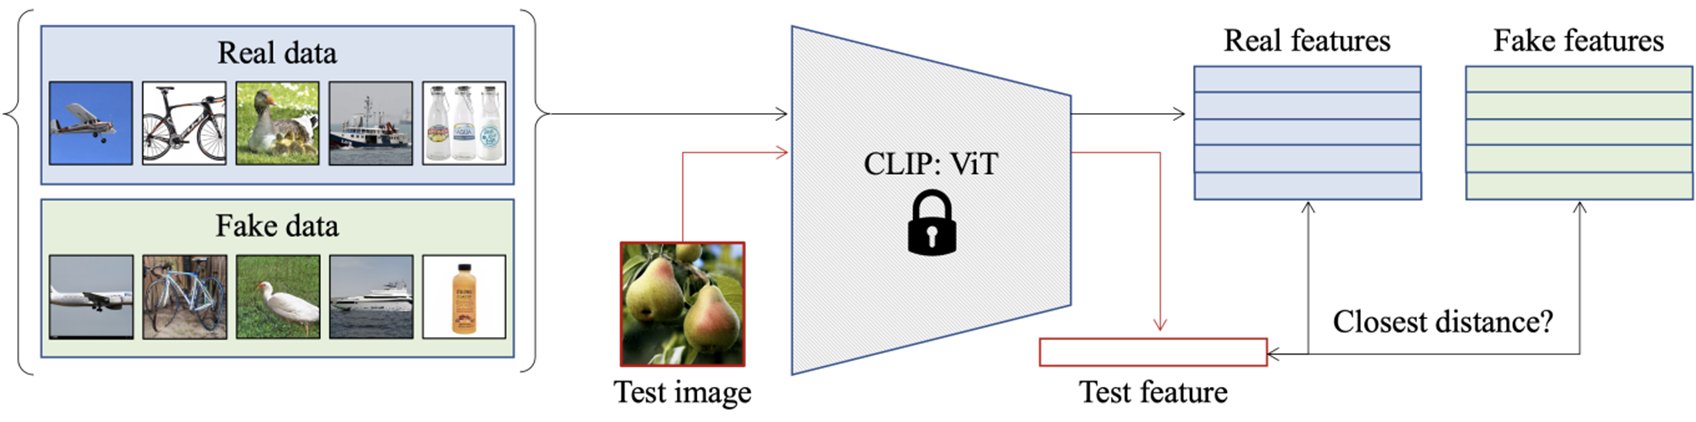
\includegraphics[width=0.8\textwidth]{Images/method_paper2.png}
    \caption{Towards Universal Fake Image Detectors Nearest neighbors method for real-vs-fake image classification (Paper 2)}
    \label{fig:methodology}
\end{figure}
The linear classification method involves layering a single linear layer with sigmoid activation on top of the CLIP encoder. Only this new classification layer is trained using binary cross-entropy loss for binary real-vs-fake classification. While being more computationally efficient, this method preserves the benefits of the nearest neighbor method by training a limited number of parameters in the linear layer. All things considered, the methodology presents a promising approach for fake image detection by using an untrained feature space derived from CLIP to distinguish between real and fake images.
\vspace{1cm}
\section{Paper 3: Fake-image detection with Robust Hashing}
This paper has suggested a technique for robust hashing-based fake-image detection that provides an easy-to-use yet efficient way to discriminate between actual and altered photos. Using a particular hashing technique, the methodology computes resilient hash values from reference photos and stores them in a database. In a similar manner, hash values from query photos are calculated and compared to database information. Whether a picture is considered legitimate or false depends on how far its hash value differs from those in the database. This work employs a robust hashing method that consists of several steps: image scaling, rich feature extraction, Gaussian low-pass filtering, and bit string output as the hash value.
\begin{figure}[H]
    \centering
    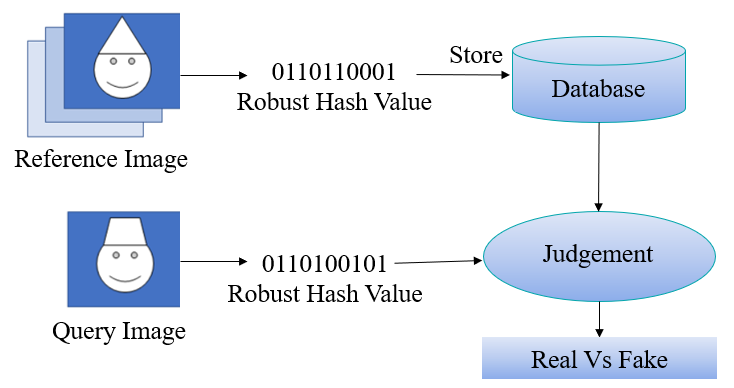
\includegraphics[width=0.8\textwidth]{Images/method_paper3.png}
    \caption{Robust Hashing Method (Paper 3)}
    \label{fig:data_transformation}
\end{figure}
The experimental evaluation made use of four fake-image datasets: the Image Manipulation Dataset, UADFV, CycleGAN, and StarGAN \cite{10} \cite{18}. JPEG compression was used for all query photos, and a threshold value was selected based on Equal Error Rate performance. The proposed method was compared with Wang et al.'s state-of-the-art fake detection method, which focuses on CNN-generated image identification. The experimental results demonstrate that the suggested method works better than Wang's method in terms of Average Precision (AP) and Accuracy (fake), particularly when working with datasets that entail picture change. All things considered, the proposed method exhibits potential for detecting fake images and offers protection against various forms of picture manipulation.
\vspace{5cm}
\section{Comparison of Three Papers}
\vspace{0.5cm}
\textbf{Paper 1: Non-local Attention based Fake Image Detection (NAFID) network}
\begin{itemize}
    \item Non-local features are extracted using the NFE module
    \item Probability density function (PDF) of PSNR values after denoising for real and fake images are calculated
    \item ResNeXt is adopted as the classification network to distinguish real and fake images
\end{itemize}
\vspace{0.5cm}
\textbf{Paper 2: CLIP:ViT network (Visual Transformer within Contrastive Language-Image Pre-training \cite{2})}
\begin{itemize}
    \item Feature Space Selection using ViT-L/14 with patch size 14x14
    \item Cosine distance is calculated to find the nearest neighbors to both real and fake feature banks
    \item Two simple classification methods are investigated: nearest neighbor and linear probing
\end{itemize}
\vspace{0.5cm}
\textbf{Paper 3: Robust Hashing Method (robust hash value stored into  database)}
\begin{itemize}
    \item Robust hash value calculated by resizing images to 128x128 pixels, applying 5x5 Gaussian low-pass filtering
    \item Hamming distance calculation between their hash strings
    \item Thresholding to determine if the query image is fake or not
\end{itemize}

\chapter{Result Analysis}
From paper 1 network; NAFID \cite{1}, detects phony faces. Compared to state-of-the-art approaches, NAFID outperforms them on a variety of forgeries datasets with impressive detection accuracy, particularly on datasets featuring complex GAN structures such as StyleGAN2. NAFID's efficacy stems from its capacity to efficiently extract non-local features, as evidenced by the enhancement it confers upon previous models for forgery detection.\\
\begin{figure}[H]
    \centering
    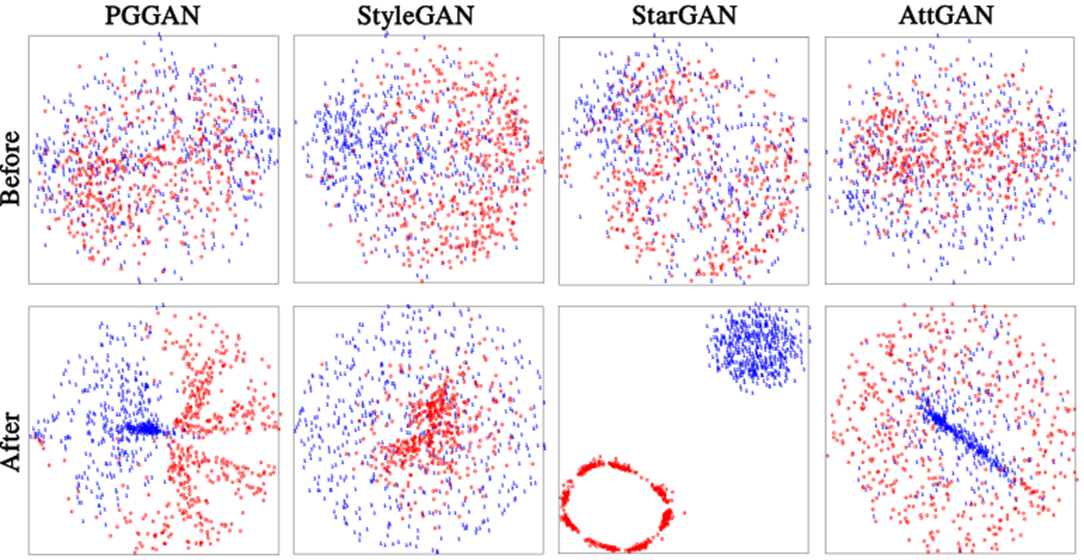
\includegraphics[width=0.8\textwidth]{Images/result_paper1.png}
    \caption{Before and after distributions of real/fake features 
    visualized by t-SNE using NFE module (Paper 1)}
    \label{fig:data_transformation}
\end{figure}
The usefulness of the non-local feature extraction module in distinguishing between actual and fake images is further confirmed by the visualization results obtained using t-SNE and Grad-CAM. The design and success of NAFID are based on a fundamental insight: fake faces have stronger non-local self-similarity than real ones.\\
\\
\\
\\
\\
\\
\\
Paper 2 has evaluated several approaches to false picture detection, emphasizing the transferability of these approaches to various generative model types. Conventional deep neural networks have difficulty with generalization and occasionally categorize undetectable false visuals erroneously. But the suggested approach makes use of a pre-trained network's feature space to achieve far higher generalization performance and keeps high accuracy even when used with unidentified generative models. Experiments also reveal that altering the pre-training dataset or backbone design has a considerable impact on the detection efficacy; models trained on a wider variety of datasets perform better.
\begin{figure}[H]
    \centering
    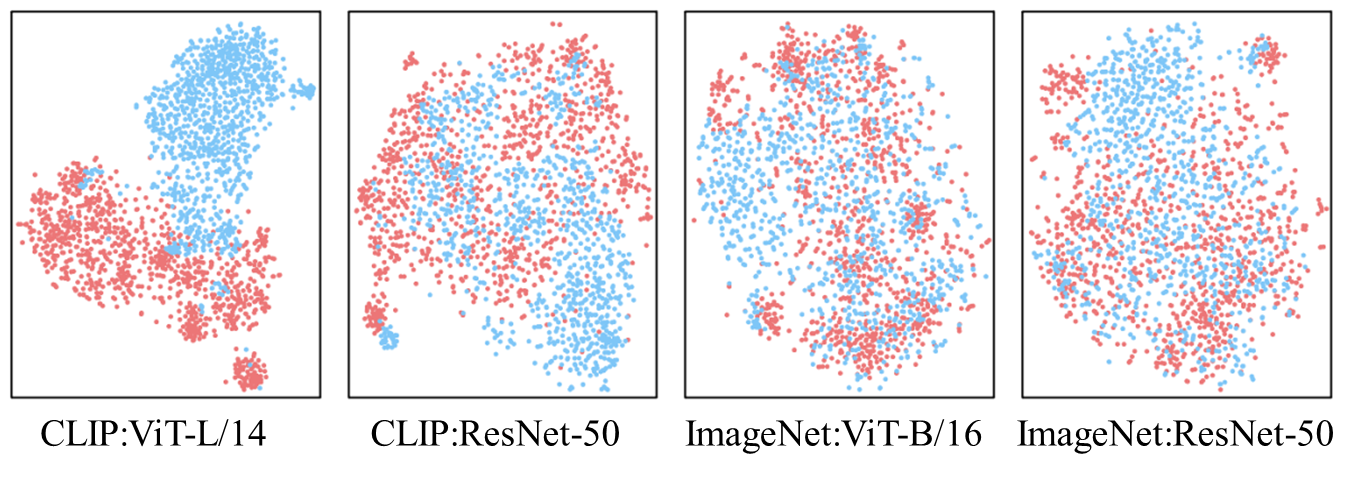
\includegraphics[width=0.8\textwidth]{Images/result_paper2.png}
    \caption{Before and after distributions of real/fake features visualized\\ by t-SNE of feature space of different image encoders using nearest neighbors (Paper 2)}
    \label{fig:data_transformation}
\end{figure}
Furthermore, the model can still achieve strong generalizability when multiple training data sources, such as ProGAN or LDM, are used. This suggests a latent relationship between different kinds of false pictures. In general, the findings emphasize how crucial it is to use pre-trained feature spaces for reliable false picture identification, particularly in generative model landscapes that are varied and dynamic.\\
\\
\\
\\
\\
The experimental results for paper 3 demonstrates that the proposed method outperforms Wang's method in terms of Average Precision (AP) and Accuracy (fake) on a range of datasets, including those requiring picture alteration. Specifically, when working with datasets like Image Manipulation Dataset and UADFV, where images are manipulated using methods other than GANs, Wang's method performs significantly worse than the recommended approach. This demonstrates that the recommended approach can withstand a wider range of image modifications.
\begin{figure}[H]
    \centering
    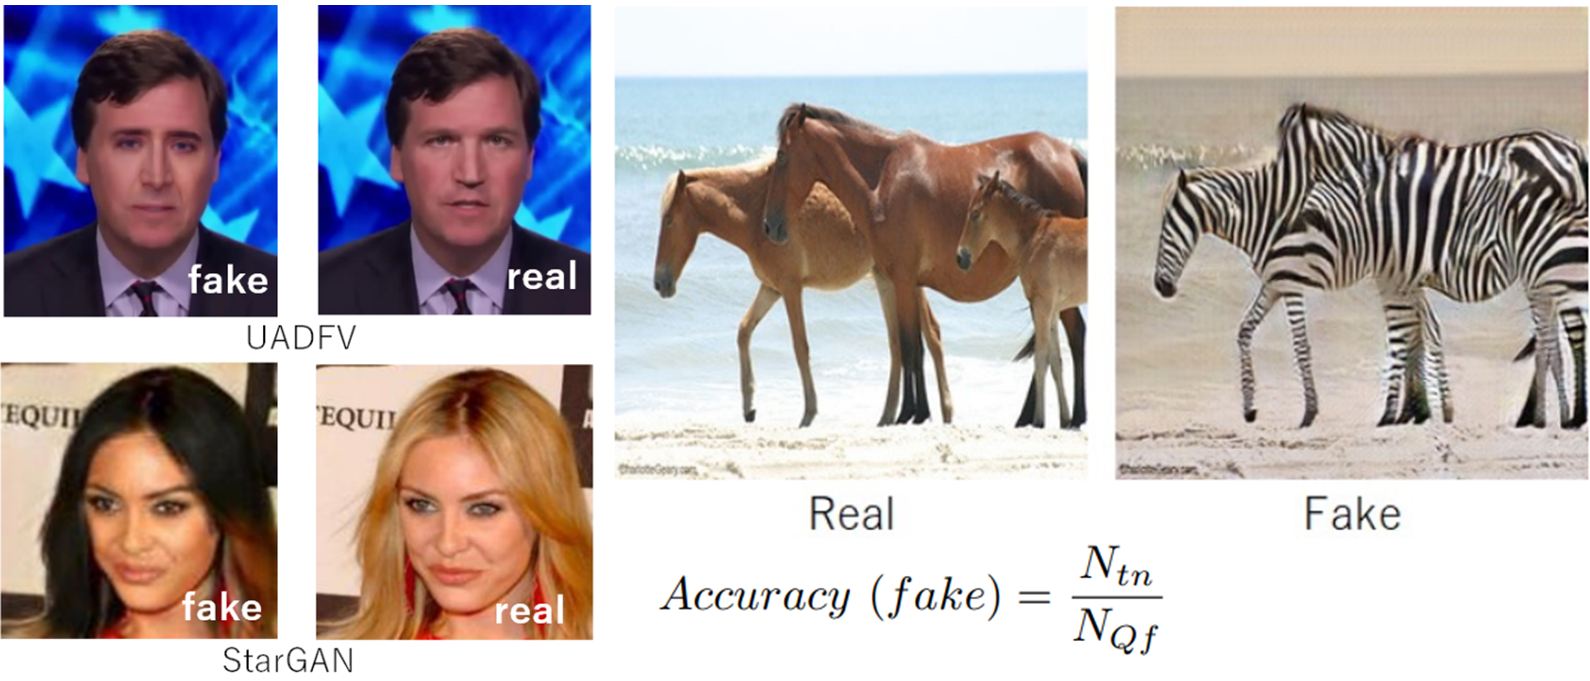
\includegraphics[width=0.8\textwidth]{Images/result_paper3.png}
    \caption{Some Outputs from Robust Method}
    \label{fig:data_transformation}
\end{figure}
Furthermore, Wang's method performs poorly, especially when conducting operations like splicing and resizing, while the suggested strategy maintains great accuracy under additional manipulations like JPEG compression, resizing, copy-move, and splicing. This discrepancy stems from Wang's methodology, which focuses on identifying unique characteristics introduced by CNNs and is independent of splicing and resizing processes. Conversely, the robust hashing strategy of the proposed method demonstrates its versatility and effectiveness in detecting fake photographs by enabling it to recognize them using a variety of altering techniques.

\begin{table}[H]
    \centering
    \caption{Quantitative evaluation results on test 1000 dataset}
    \label{tab:results_test_1000}
    \begin{tabular}{|c|c|c|c|}
        \hline
        \textbf{Methods} & \textbf{PGGAN} &\textbf{StyleGAN} &\textbf{StyleGAN2}\\ \hline
        NAFID & 100.00 & 99.68 & 99.07 \\ \hline
        CLIP:ViT & - & 97.24 & -  \\ \hline
        Robust Hashing & - & - & - \\ \hline
        \hline
        \textbf{Methods} & \textbf{StarGAN} &\textbf{Deepfakes} &\textbf{CycleGAN}\\ \hline
        NAFID & 100.00 & 98.74 & - \\ \hline
        CLIP:ViT & 99.60 & 93.09 & 99.46  \\ \hline
        Robust Hashing & 100.00 & - & 100.00 \\ \hline
    \end{tabular}
\end{table}
From this table, it is clear that method 1 and method 3 are dominating over method 2 in case of numerical result analysis. Among them method 1 has given better results as it is tested on most of the different sets of test cases.

\chapter{Findings and Recommendations}
\section{Findings}
\textbf{Paper 1 Findings: NAFID Network}
\begin{itemize}
    \item Observation on compared to actual faces, artificial faces show more non-local self-similarity
    \item Suggestion of a non-local feature extraction (NFE) module in light of this observation in order to extract non-local features from fictitious faces
    \item Method's efficacy is confirmed on multiple forgeries datasets, exhibiting a consistent high performance
\end{itemize}
\textbf{Paper 2 Findings: CLIP:ViT Network}
\begin{itemize}
    \item More diverse datasets, such as CLIP, produce better generalization than ImageNet-like datasets
    \item The training data source has an effect on generalizability; generative models trained on a range of datasets perform better
\end{itemize}
\textbf{Paper 3 Findings: Robust Hashing}
\begin{itemize}
    \item When compared to baselines that are currently in use, the suggested robust hashing algorithm performs better at differentiating between actual and fraudulent photos
    \item When confronted with images from unknown generative models, traditional deep neural networks exhibit notable reductions in accuracy, incorrectly recognizing a large number of bogus images as real
\end{itemize}
\vspace{0.5cm}
\section{Recommendations}
\vspace{0.5cm}
\begin{itemize}
    \item In case of NAFID Network, Additional testing on bigger and more varied datasets to evaluate the suggested method's resilience in different situations and investigating different methods or architectures to improve detection performance, particularly in difficult situations such as identifying phony photos from hidden generative models.
    \vspace{0.5cm}
    \item In case of Clip-ViT, how well CLIP scales to handle larger and more diverse datasets, particularly in domains other than picture classification looking for ways to improve CLIP such that its cross-domain generality is preserved when it is used for specific downstream tasks.
    \vspace{0.5cm}
    \item In case of Robust Hashing method, testing the method's robustness by doing tests to see how well it works with various image distortions and modifications and investigating uses for strong hashing techniques that go beyond the identification of false images, such as content-based picture retrieval or digital forensics tamper detection
    \vspace{0.5cm}
    \item In case of NAFID method, evaluation on six fake face datasets with 9K training images which is quite difficult comparing to other methods
    \vspace{0.5cm}
    \item Concerns regarding future image generation technology improvements
    \vspace{0.5cm}
    \item Above all, seeing the result analysis comparing three methods, NAFID method seems to be the optimal solution among them due to accuracy and variability of test cases
\end{itemize}

\chapter{Addressing Course Outcomes and Program Outcomes}
\textbf{Problem Analysis:}
Problem analysis is used in the seminar lab presentation to thoroughly examine the difficulties in identifying phony photos in a variety of datasets and generative models. Examined are a number of variables that impact the precision and dependability of current detection systems, such as differences in image quality, generative model complexity, and the existence of advanced forgery techniques.\\
\textbf{Ethics:}
Plagiarism-related concerns and ethical considerations are given careful attention in the seminar lab presentation. The topic of debate centers on the moral ramifications of producing and sharing false images, highlighting the possible harm these images may do to people as well as to society. The need of following ethical norms and using appropriate citation techniques is emphasized as a way to guarantee ethical behavior. In this lab, plagiarism is strongly condemned and dealt with. The necessity of upholding originality and academic integrity in research and presentations is brought to the audience's attention. In order to guarantee that any content offered is sourced responsibly and acknowledged, plagiarism prevention techniques are addressed. These include accurately citing references and providing a data summary. \\
\textbf{Individual and Teamwork:}
The value of both individual and team contributions is stressed in the seminar lab presentation. The distinct abilities and knowledge of each member are recognized, and teamwork is encouraged to accomplish shared objectives. In order to promote a harmonious and effective team environment, teamwork techniques including task delegation, effective communication, and conflict resolution are covered.\\
\textbf{Communication:}
In any kind of presentation, clear and succinct information delivery is prioritized as an essential component of effective communication. To make sure that everyone gets the message, emphasis is placed on effective communication techniques like articulation, audience involvement, and active listening. Feedback systems are meant to encourage candid communication and helpful criticism among team members, promoting understanding and ongoing development.

\chapter{Addressing Complex Engineering Activities}

Handling complicated engineering tasks entails using sophisticated technical expertise and problem-solving techniques to take on challenging tasks across a range of industries. This can include creating complex system designs, streamlining procedures, carrying out in-depth assessments, and coming up with creative fixes in case of complex engineering activities.
\\
\\
\\
\textbf{Range of Resources:}
\\
A variety of tools are used to improve the efficacy of communication, including visual aids like slideshows and charts to support spoken explanations. Written materials are also supplied, such as reports or handouts, to give the audience extensive information and points of reference. Digital platforms can also be used for document or presentation sharing and distant collaboration. These varied materials accommodate various learning preferences and improve audience comprehension and participation during the presentation.
\\
\\
\\
\textbf{Level of Interaction:}
\\
There is a lot of interaction encouraged during the presentation, which motivates the audience to actively participate and become involved. In order to promote communication and idea exchange, there will be opportunities for questions, comments, and discussions throughout the session. Presenters actively solicit input from the audience, requesting that they share their opinions and insights on the topic at hand. Examples of interactive elements that can be used to increase engagement and foster a dynamic learning environment are polls and group activities.
\\
\\
\\
\\
\\
\\
\\
\textbf{Innovation:}
\\
The investigation of original concepts, inventive methods to problem-solving, and the creation of ground-breaking solutions all promote innovation. There is a focus on thinking creatively, questioning accepted wisdom, and expanding the frontiers of technology and knowledge. Diverse viewpoints are encouraged to drive innovation through collaboration and cross-disciplinary communication. Furthermore, a culture of experimentation and risk-taking is fostered to motivate people and groups to investigate novel avenues and grasp prospects for growth.
\\
\\
\\
\\
\textbf{Concequences for Society and the Environment:}
\\
The potential consequences of innovation and technical breakthroughs are carefully addressed in order to guarantee that society and the environment are improved. This entails evaluating how new innovations might affect different stakeholders, such as communities, ecosystems, and the coming generation. Unwanted outcomes that are lessened by legislation include social unrest, environmental destruction, and economic inequality. Sustainable techniques are included into decision-making processes to reduce environmental impact and enhance resource efficiency. In addition, ethical issues influence the adoption and use of technologies to guarantee that they respect social norms and safeguard human rights. Generally speaking, an all-encompassing strategy that strikes a balance between progress and social and environmental obligations is employed to build a more just and sustainable society.
\\
\\
\\
\textbf{Familarity:}
\\
The degree of knowledge or comprehension that people has on a specific subject, idea, or circumstance is referred to as familiarity. It includes the extent to which people are able to identify, comprehend, or feel something. People's levels of familiarity with a subject matter can differ depending on their experiences, education, backgrounds, and exposure to it. It has a significant impact on how people interact with and react to tasks, information, or difficulties, which affects how they make decisions and behave. Gaining more knowledge about a subject often results in an increase in one's self-assurance, skill, and productivity when handling related problems or assignments. And so, familarity with information has been understood throughout this lab.

\chapter{Conclusion}
In conclusion, a variety of generative models and datasets have demonstrated the effectiveness of the NAFID framework, a revolutionary approach to false image detection. By employing multi-stage classification and non-local feature extraction algorithms, NAFID consistently achieves great levels of accuracy, even on challenging datasets such as StyleGAN2. Its capacity to distinguish between real and fake photos with such accuracy demonstrates how flexible and robust the method is. Similarly, CLIP is a notable invention because of its remarkable generalization capacity, which allows it to cohesively bridge the gap between images and natural words. Comprehending visual and textual inputs is essential for numerous multimodal AI applications, as this ability carries significant benefits. Furthermore, because of its compact and discriminative picture representation, the robust hashing approach is an attractive alternative. It is a useful tool in the toolkit of image authentication techniques due to its resistance to frequent alterations and efficiency in identifying phony photos in a variety of scenarios. Together, these results demonstrate how these techniques could have a big impact on the field of picture forensics and inspire more study to improve and expand their usefulness.
Among three different approaches, Non-local Attention based Fake Image Detection (NAFID) network using NFE module is the optimal one. NAFID \cite{1} has (99-100)\% accuracy in most of the GAN based test cases and so it works best on GAN or AI generated images 
Further exploration and validation could enhance the appropriateness of these methods in real-world scenarios.

\renewcommand{\bibname}{References}
\bibliographystyle{plain} % Choose a bibliography style
\bibliography{sample} % The name of your .bib file

\chapter{Publication Details}
\begin{figure}[H]
    \centering
    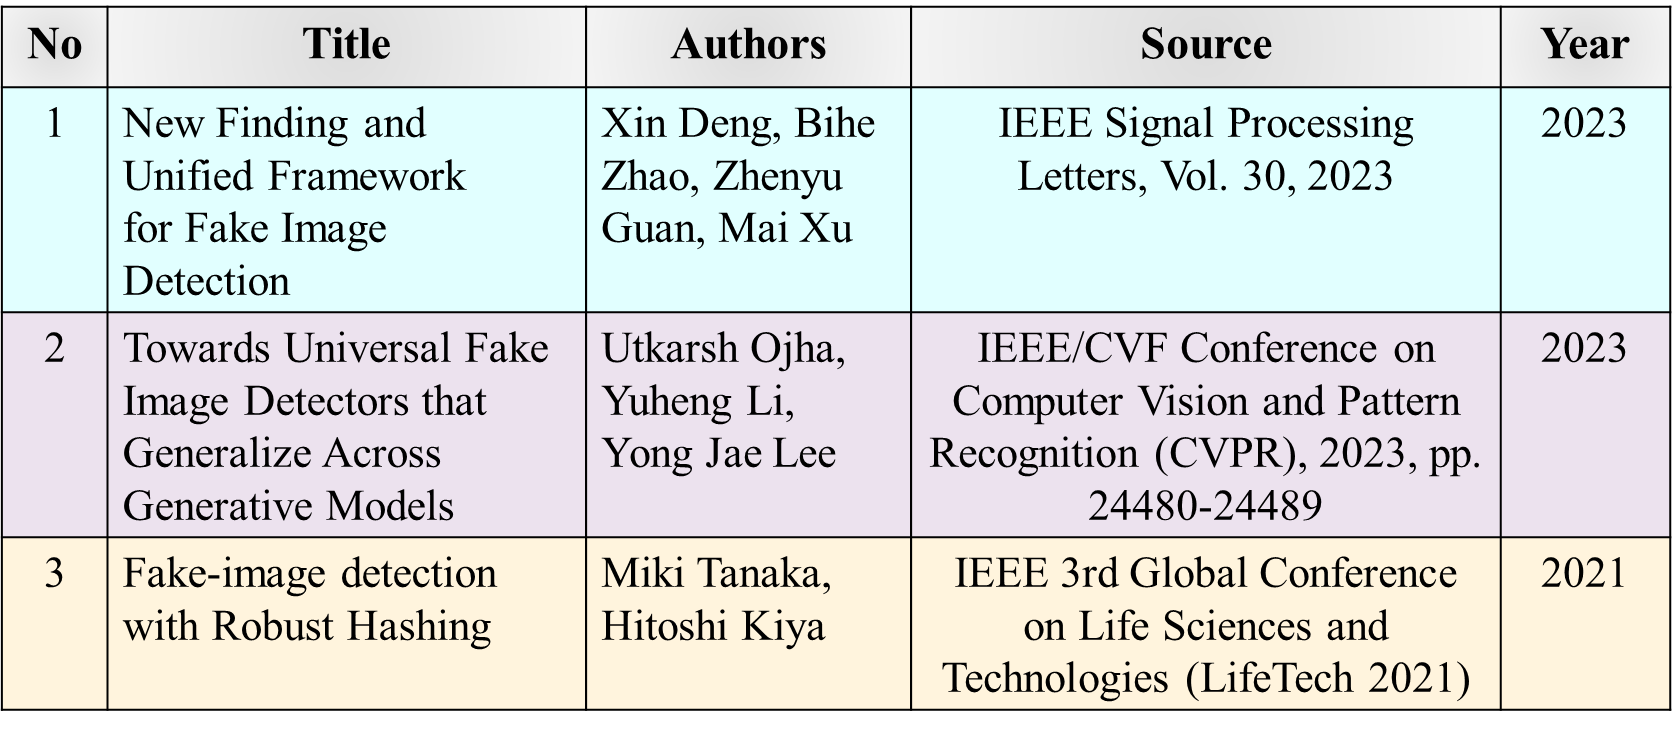
\includegraphics[width=1\textwidth]{Images/publications.png}
    \caption{Publication details of three papers}
    \label{fig:rainy_clean}
\end{figure}
All three of the papers have been attached next after this page for more precision.

\end{document}
